\documentclass[]{book}
\usepackage{lmodern}
\usepackage{amssymb,amsmath}
\usepackage{ifxetex,ifluatex}
\usepackage{fixltx2e} % provides \textsubscript
\ifnum 0\ifxetex 1\fi\ifluatex 1\fi=0 % if pdftex
  \usepackage[T1]{fontenc}
  \usepackage[utf8]{inputenc}
\else % if luatex or xelatex
  \ifxetex
    \usepackage{mathspec}
  \else
    \usepackage{fontspec}
  \fi
  \defaultfontfeatures{Ligatures=TeX,Scale=MatchLowercase}
\fi
% use upquote if available, for straight quotes in verbatim environments
\IfFileExists{upquote.sty}{\usepackage{upquote}}{}
% use microtype if available
\IfFileExists{microtype.sty}{%
\usepackage{microtype}
\UseMicrotypeSet[protrusion]{basicmath} % disable protrusion for tt fonts
}{}
\usepackage[margin=1in]{geometry}
\usepackage{hyperref}
\hypersetup{unicode=true,
            pdftitle={bdclean User Guide},
            pdfauthor={Authors: Tomer Gueta and Thiloshon Nagarajah},
            pdfborder={0 0 0},
            breaklinks=true}
\urlstyle{same}  % don't use monospace font for urls
\usepackage{natbib}
\bibliographystyle{apalike}
\usepackage{color}
\usepackage{fancyvrb}
\newcommand{\VerbBar}{|}
\newcommand{\VERB}{\Verb[commandchars=\\\{\}]}
\DefineVerbatimEnvironment{Highlighting}{Verbatim}{commandchars=\\\{\}}
% Add ',fontsize=\small' for more characters per line
\usepackage{framed}
\definecolor{shadecolor}{RGB}{248,248,248}
\newenvironment{Shaded}{\begin{snugshade}}{\end{snugshade}}
\newcommand{\KeywordTok}[1]{\textcolor[rgb]{0.13,0.29,0.53}{\textbf{#1}}}
\newcommand{\DataTypeTok}[1]{\textcolor[rgb]{0.13,0.29,0.53}{#1}}
\newcommand{\DecValTok}[1]{\textcolor[rgb]{0.00,0.00,0.81}{#1}}
\newcommand{\BaseNTok}[1]{\textcolor[rgb]{0.00,0.00,0.81}{#1}}
\newcommand{\FloatTok}[1]{\textcolor[rgb]{0.00,0.00,0.81}{#1}}
\newcommand{\ConstantTok}[1]{\textcolor[rgb]{0.00,0.00,0.00}{#1}}
\newcommand{\CharTok}[1]{\textcolor[rgb]{0.31,0.60,0.02}{#1}}
\newcommand{\SpecialCharTok}[1]{\textcolor[rgb]{0.00,0.00,0.00}{#1}}
\newcommand{\StringTok}[1]{\textcolor[rgb]{0.31,0.60,0.02}{#1}}
\newcommand{\VerbatimStringTok}[1]{\textcolor[rgb]{0.31,0.60,0.02}{#1}}
\newcommand{\SpecialStringTok}[1]{\textcolor[rgb]{0.31,0.60,0.02}{#1}}
\newcommand{\ImportTok}[1]{#1}
\newcommand{\CommentTok}[1]{\textcolor[rgb]{0.56,0.35,0.01}{\textit{#1}}}
\newcommand{\DocumentationTok}[1]{\textcolor[rgb]{0.56,0.35,0.01}{\textbf{\textit{#1}}}}
\newcommand{\AnnotationTok}[1]{\textcolor[rgb]{0.56,0.35,0.01}{\textbf{\textit{#1}}}}
\newcommand{\CommentVarTok}[1]{\textcolor[rgb]{0.56,0.35,0.01}{\textbf{\textit{#1}}}}
\newcommand{\OtherTok}[1]{\textcolor[rgb]{0.56,0.35,0.01}{#1}}
\newcommand{\FunctionTok}[1]{\textcolor[rgb]{0.00,0.00,0.00}{#1}}
\newcommand{\VariableTok}[1]{\textcolor[rgb]{0.00,0.00,0.00}{#1}}
\newcommand{\ControlFlowTok}[1]{\textcolor[rgb]{0.13,0.29,0.53}{\textbf{#1}}}
\newcommand{\OperatorTok}[1]{\textcolor[rgb]{0.81,0.36,0.00}{\textbf{#1}}}
\newcommand{\BuiltInTok}[1]{#1}
\newcommand{\ExtensionTok}[1]{#1}
\newcommand{\PreprocessorTok}[1]{\textcolor[rgb]{0.56,0.35,0.01}{\textit{#1}}}
\newcommand{\AttributeTok}[1]{\textcolor[rgb]{0.77,0.63,0.00}{#1}}
\newcommand{\RegionMarkerTok}[1]{#1}
\newcommand{\InformationTok}[1]{\textcolor[rgb]{0.56,0.35,0.01}{\textbf{\textit{#1}}}}
\newcommand{\WarningTok}[1]{\textcolor[rgb]{0.56,0.35,0.01}{\textbf{\textit{#1}}}}
\newcommand{\AlertTok}[1]{\textcolor[rgb]{0.94,0.16,0.16}{#1}}
\newcommand{\ErrorTok}[1]{\textcolor[rgb]{0.64,0.00,0.00}{\textbf{#1}}}
\newcommand{\NormalTok}[1]{#1}
\usepackage{longtable,booktabs}
\usepackage{graphicx,grffile}
\makeatletter
\def\maxwidth{\ifdim\Gin@nat@width>\linewidth\linewidth\else\Gin@nat@width\fi}
\def\maxheight{\ifdim\Gin@nat@height>\textheight\textheight\else\Gin@nat@height\fi}
\makeatother
% Scale images if necessary, so that they will not overflow the page
% margins by default, and it is still possible to overwrite the defaults
% using explicit options in \includegraphics[width, height, ...]{}
\setkeys{Gin}{width=\maxwidth,height=\maxheight,keepaspectratio}
\IfFileExists{parskip.sty}{%
\usepackage{parskip}
}{% else
\setlength{\parindent}{0pt}
\setlength{\parskip}{6pt plus 2pt minus 1pt}
}
\setlength{\emergencystretch}{3em}  % prevent overfull lines
\providecommand{\tightlist}{%
  \setlength{\itemsep}{0pt}\setlength{\parskip}{0pt}}
\setcounter{secnumdepth}{5}
% Redefines (sub)paragraphs to behave more like sections
\ifx\paragraph\undefined\else
\let\oldparagraph\paragraph
\renewcommand{\paragraph}[1]{\oldparagraph{#1}\mbox{}}
\fi
\ifx\subparagraph\undefined\else
\let\oldsubparagraph\subparagraph
\renewcommand{\subparagraph}[1]{\oldsubparagraph{#1}\mbox{}}
\fi

%%% Use protect on footnotes to avoid problems with footnotes in titles
\let\rmarkdownfootnote\footnote%
\def\footnote{\protect\rmarkdownfootnote}

%%% Change title format to be more compact
\usepackage{titling}

% Create subtitle command for use in maketitle
\newcommand{\subtitle}[1]{
  \posttitle{
    \begin{center}\large#1\end{center}
    }
}

\setlength{\droptitle}{-2em}

  \title{\texttt{bdclean} User Guide}
    \pretitle{\vspace{\droptitle}\centering\huge}
  \posttitle{\par}
    \author{Authors: Tomer Gueta and Thiloshon Nagarajah}
    \preauthor{\centering\large\emph}
  \postauthor{\par}
      \predate{\centering\large\emph}
  \postdate{\par}
    \date{2018-09-05}

\usepackage{booktabs}

\begin{document}
\maketitle

{
\setcounter{tocdepth}{1}
\tableofcontents
}
\chapter*{Introduction}\label{introduction}
\addcontentsline{toc}{chapter}{Introduction}

\texttt{bdclean} is a user-friendly data cleaning Shiny app for the
inexperienced R user. It provides features to manage complete workflow
for biodiversity data cleaning, from uploading the data; gathering input
from the user, in order to adjust cleaning procedures; perform the
cleaning; and finally, generating various reports and several versions
of the data. \texttt{bdclean} is part of
\href{https://bd-r.github.io/The-bdverse/index.html}{The bdverse} -- a
collection of tools, that form a general framework for facilitating
biodiversity science in R.

\begin{figure}
\centering
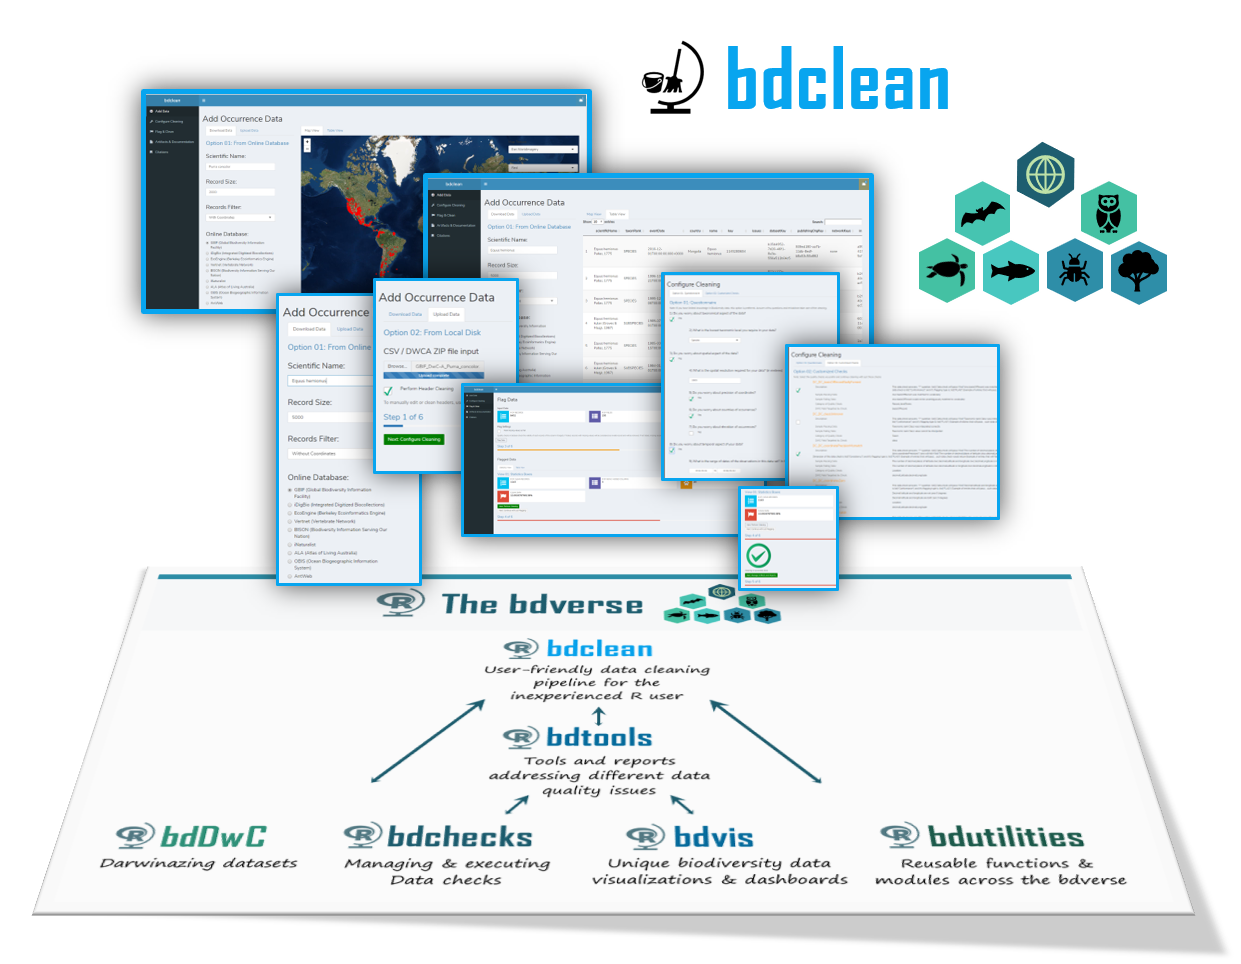
\includegraphics{img/bdclean_bdverse.png}
\caption{bdclean in the bdverse}
\end{figure}

\subsubsection*{bdclean's concept}\label{bdcleans-concept}
\addcontentsline{toc}{subsubsection}{bdclean's concept}

\begin{figure}
\centering
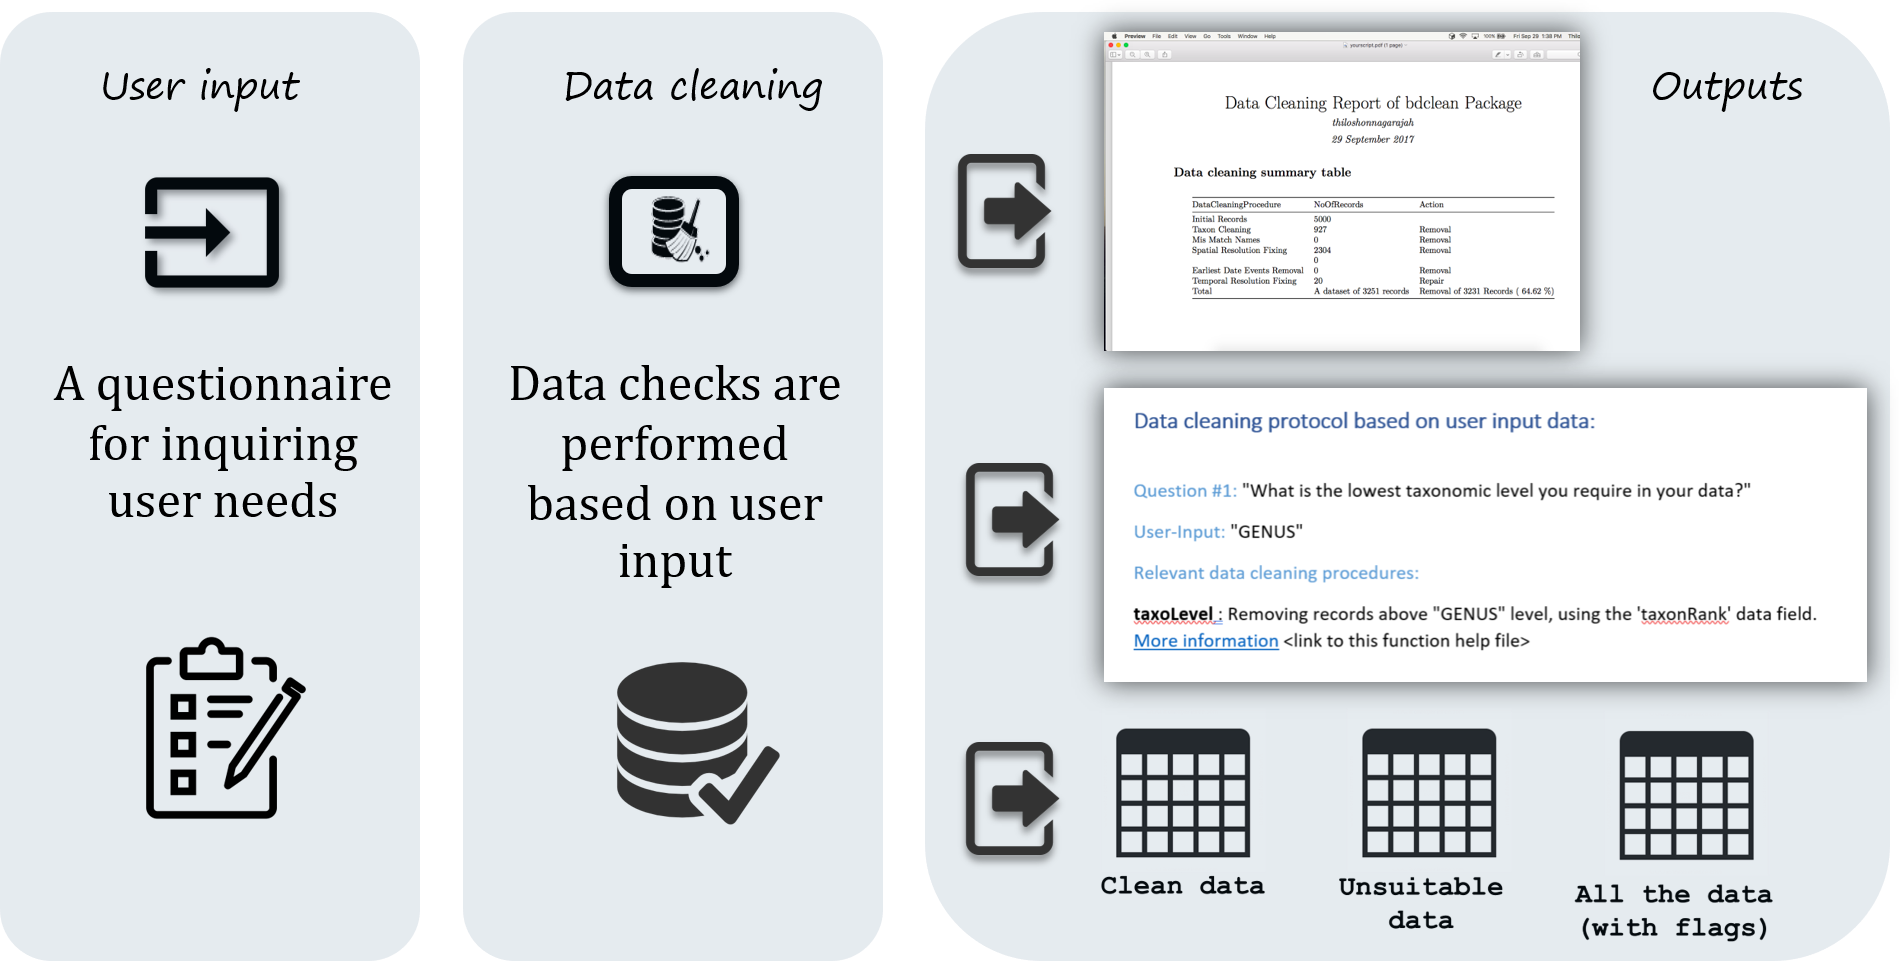
\includegraphics{img/bdclean_overview.png}
\caption{The main idea behind bdclean}
\end{figure}

bdclean workflow is comprised of three distinct mechanisms, user input,
data cleaning and outputs. In most R packages this basic workflow
(i.e.~input; processing; output) operates via an R function. Functions
are fundamental building blocks of R, and usually focus on very specific
task. Users must understand and supply the function with its mandatory
arguments (e.g.~data in the specified format, setting of various
function variables). Thus, in order to create a specific workflow, users
must write an R script, which requires reasonable programing skills.
bdclean avoids all that by creating a user-friendly Shiny app with
questionnaire that collects the necessary user input.

\subsubsection*{App overview}\label{app-overview}
\addcontentsline{toc}{subsubsection}{App overview}

\begin{figure}
\centering
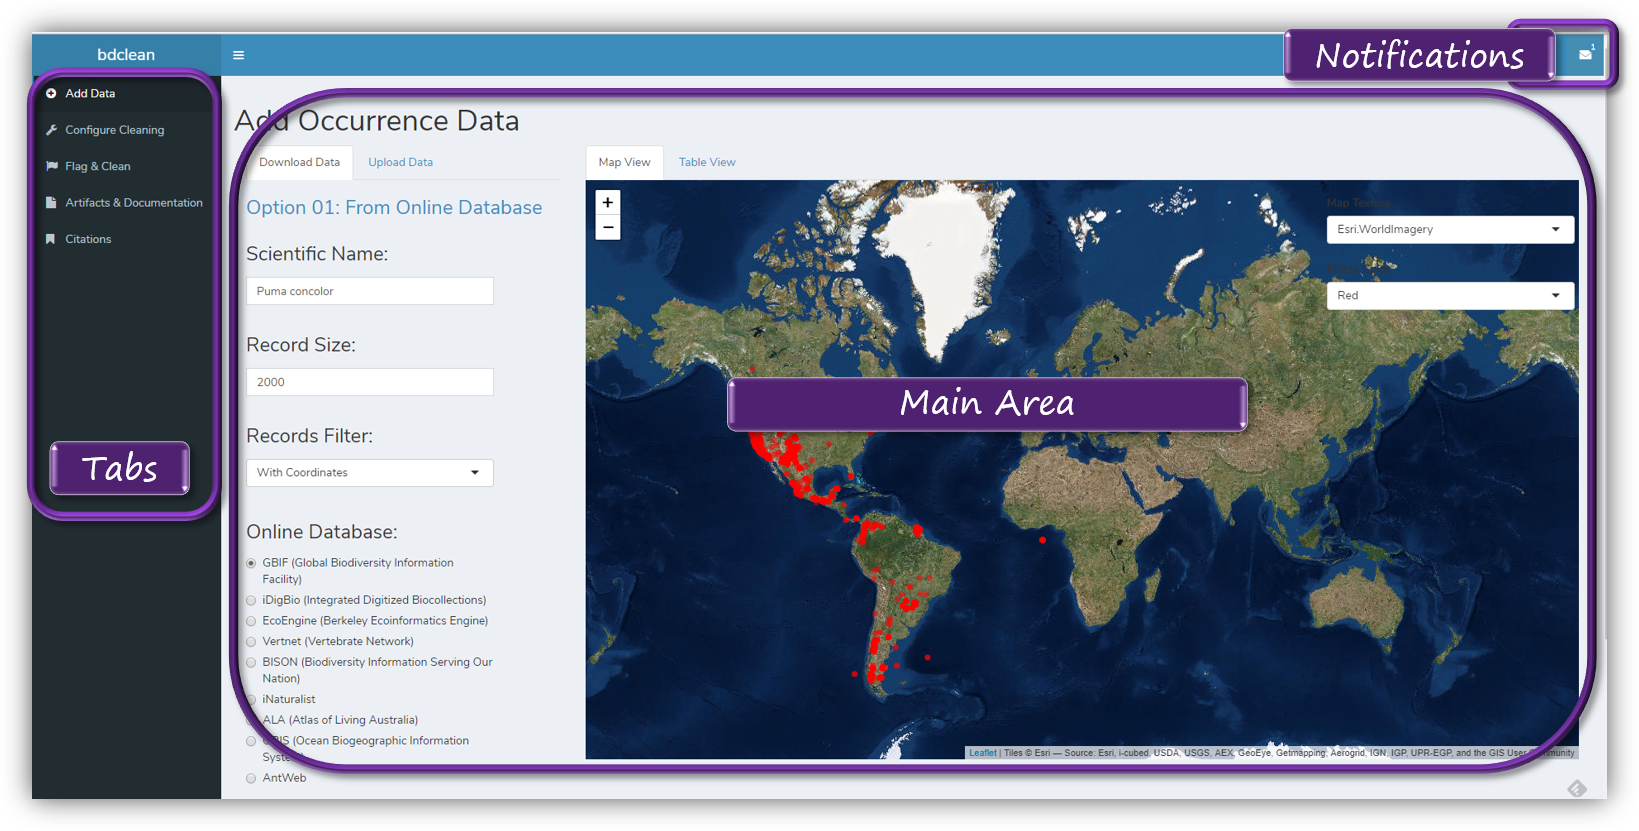
\includegraphics{img/bdclean_app_overview.png}
\caption{bdclean overview}
\end{figure}

\subsubsection*{Fundings}\label{fundings}
\addcontentsline{toc}{subsubsection}{Fundings}

\begin{figure}
\centering
\includegraphics{img/ISF.png}
\caption{}
\end{figure}

\href{https://summerofcode.withgoogle.com/\%20target=\%22_blank\%22}{\includegraphics{img/GSoC.png}}

\begin{itemize}
\tightlist
\item
  \href{https://github.com/rstats-gsoc/gsoc2018/wiki/bdclean\%3A-User-friendly-biodiversity-data-cleaning-pipeline\%20target=\%22_blank\%22}{The
  GSoC project idea page}
\end{itemize}

\chapter{\texorpdfstring{Installing
\texttt{bdclean}}{Installing bdclean}}\label{installing-bdclean}

\begin{center}\rule{0.5\linewidth}{\linethickness}\end{center}

\section{Development version from
GitHub}\label{development-version-from-github}

Windows users install
\href{https://cran.r-project.org/bin/windows/Rtools/}{Rtools} first.

\begin{Shaded}
\begin{Highlighting}[]
\KeywordTok{install.packages}\NormalTok{(}\StringTok{"devtools"}\NormalTok{)}
\NormalTok{devtools}\OperatorTok{::}\KeywordTok{install_github}\NormalTok{(}\StringTok{"bd-R/bdclean"}\NormalTok{)}
\CommentTok{# And also:}
\NormalTok{devtools}\OperatorTok{::}\KeywordTok{install_github}\NormalTok{(}\StringTok{"bd-R/bdchecks"}\NormalTok{)}
\end{Highlighting}
\end{Shaded}

\textbf{To open the Shiny app, simply run:}

\begin{Shaded}
\begin{Highlighting}[]
\KeywordTok{run_bdclean}\NormalTok{()}
\end{Highlighting}
\end{Shaded}

\section{\texorpdfstring{{Very soon: a stable version from
CRAN}}{Very soon: a stable version from CRAN}}\label{very-soon-a-stable-version-from-cran}

\begin{Shaded}
\begin{Highlighting}[]
\KeywordTok{install.packages}\NormalTok{(}\StringTok{"bdDwC"}\NormalTok{)}
\end{Highlighting}
\end{Shaded}

\section{Possible problems \&
solutions}\label{possible-problems-solutions}

\textbf{{{[} TBA {]}}}

\subsection{???}\label{section}

TBA

\subsection{????}\label{section-1}

TBA

\chapter{Add data}\label{add-data}

\begin{center}\rule{0.5\linewidth}{\linethickness}\end{center}

\section{Directly download data to the
app}\label{directly-download-data-to-the-app}

\begin{figure}
\centering
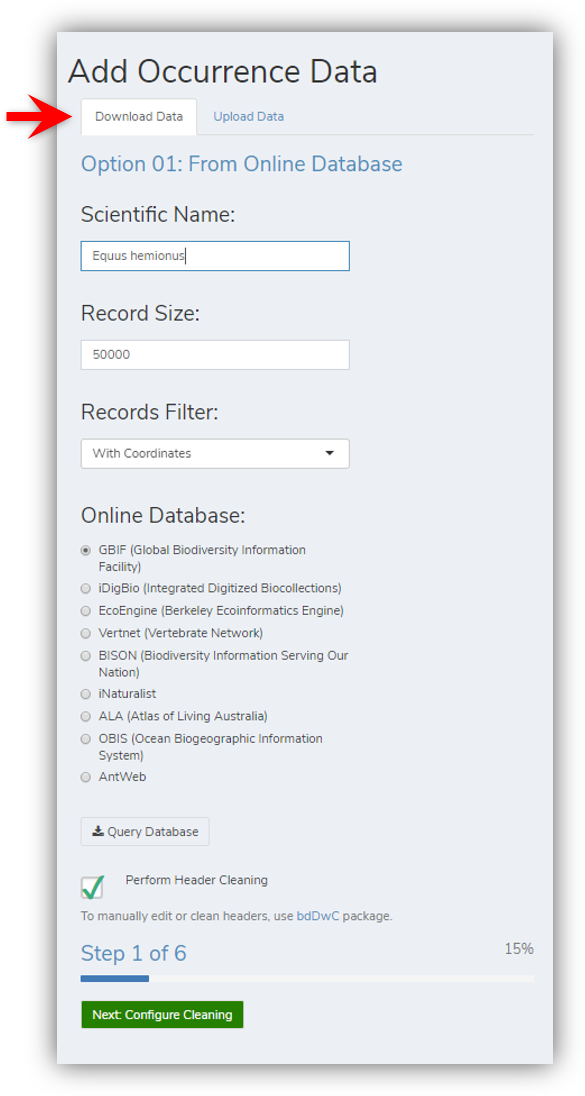
\includegraphics{img/bdclean_downlad_data.png}
\caption{Downloading data from online biodiversity databases}
\end{figure}

\textbf{OR}

\section{Upload data from a local
file}\label{upload-data-from-a-local-file}

The app supports CSV files and DwC-A zip files (Darwin Core Archive)

\begin{figure}
\centering
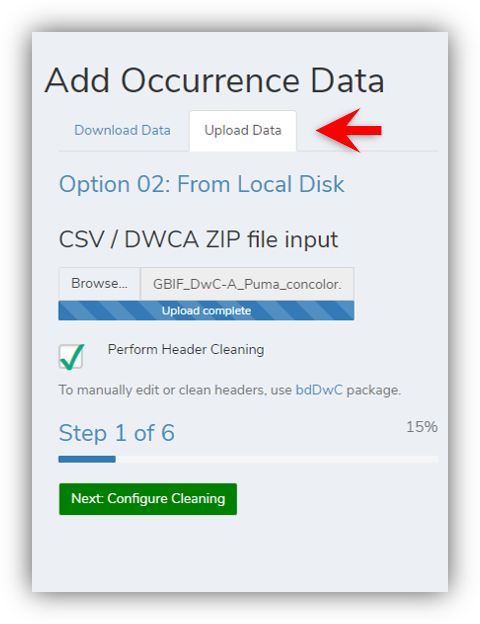
\includegraphics{img/bdclean_upload_data.png}
\caption{Upload file from a disk}
\end{figure}

\section{Map view}\label{map-view}

\begin{figure}
\centering
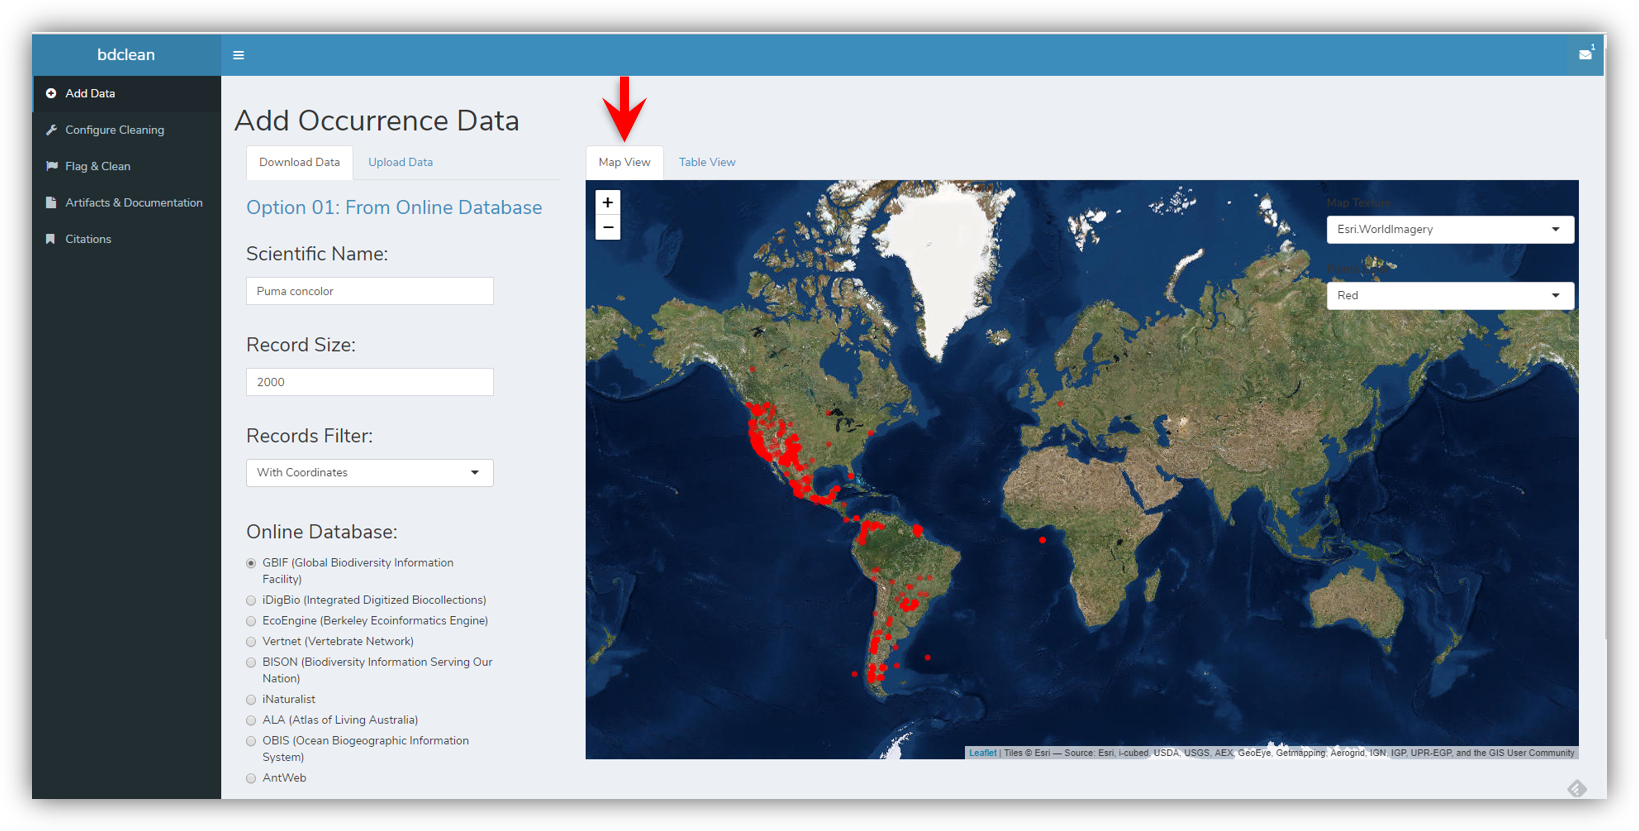
\includegraphics{img/bdclean_add_data_map.png}
\caption{View records on a map}
\end{figure}

\section{Table view}\label{table-view}

\begin{figure}
\centering
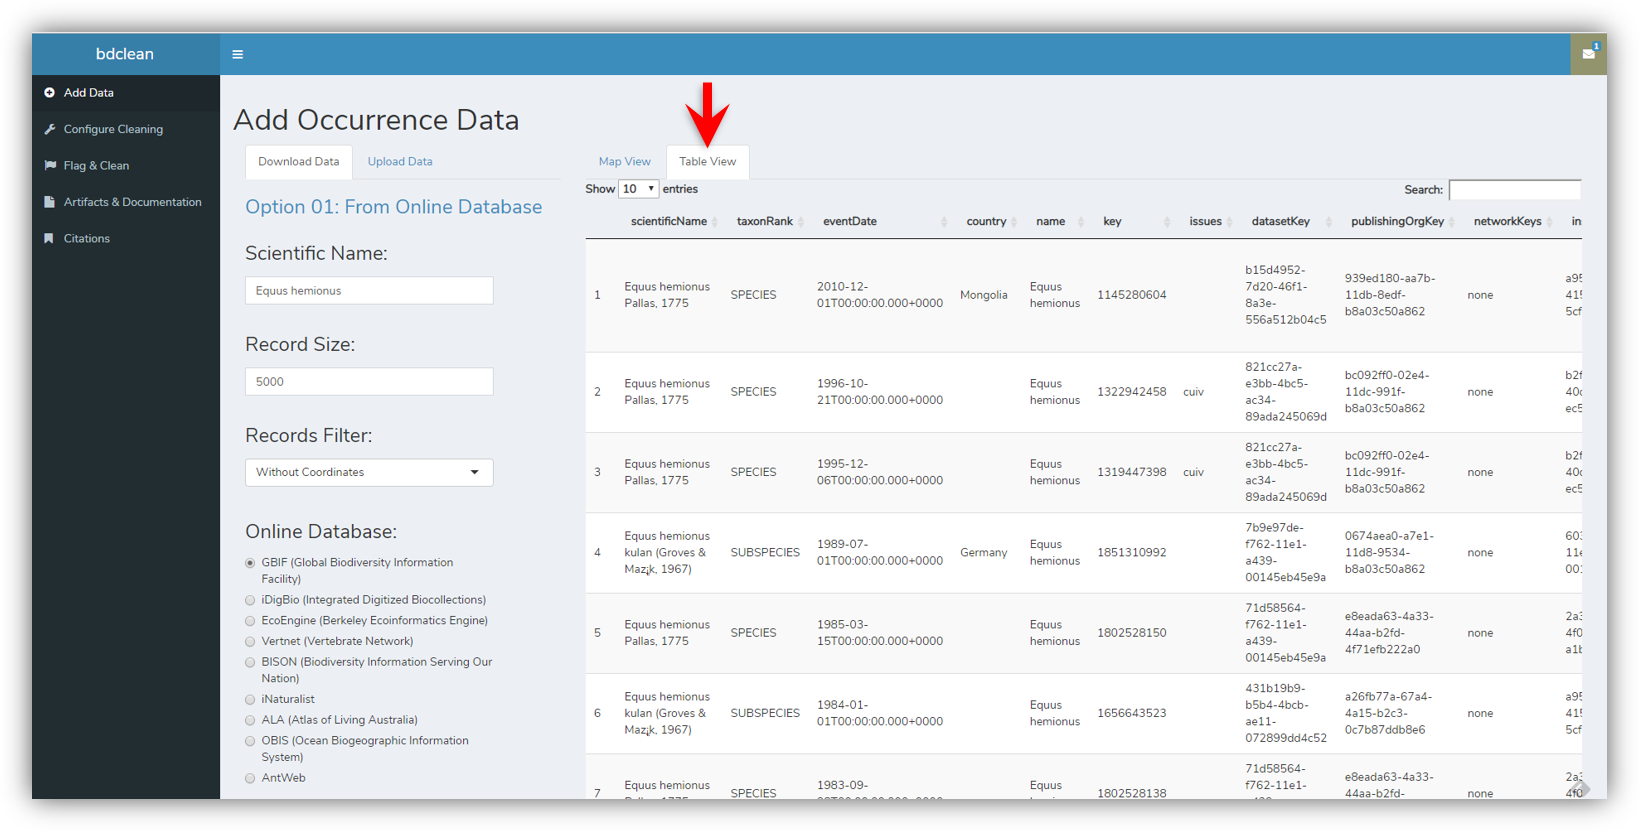
\includegraphics{img/bdclean_add_data_table.png}
\caption{View records in a table}
\end{figure}

\chapter{Data cleaning configuration}\label{data-cleaning-configuration}

\begin{center}\rule{0.5\linewidth}{\linethickness}\end{center}

\section{Option 1: a questionnaire}\label{option-1-a-questionnaire}

\begin{figure}
\centering
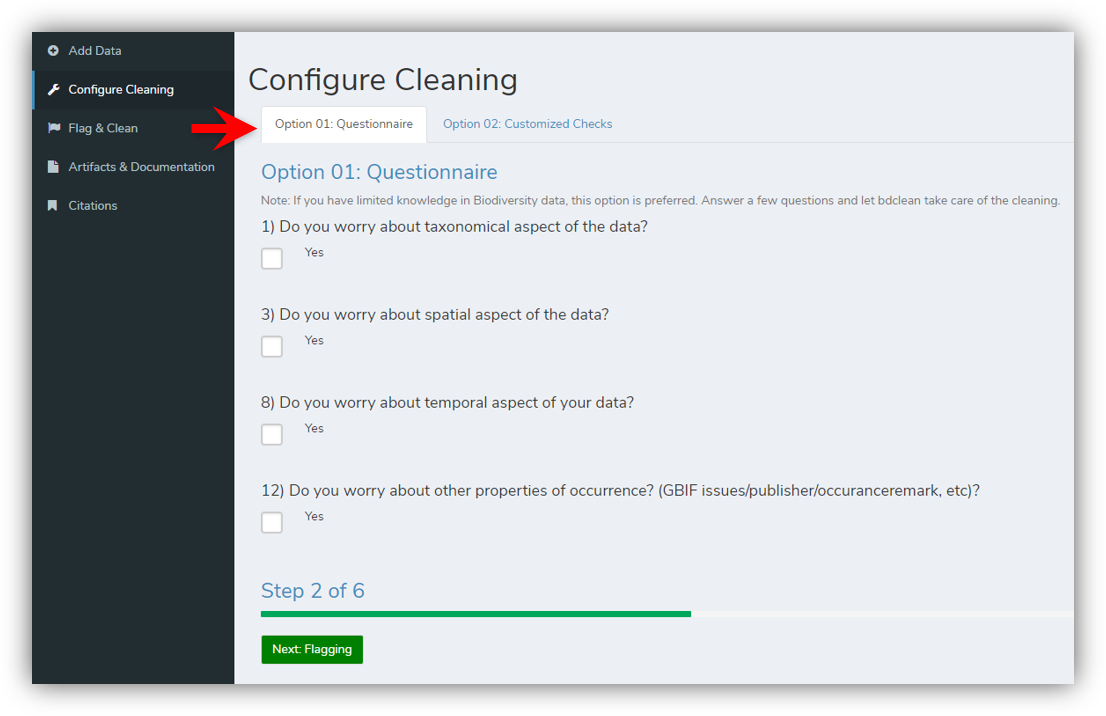
\includegraphics{img/bdclean_questionnaire-empty.png}
\caption{Data cleaning questionnaire}
\end{figure}

The questionnaire is reactive and more questions will be shown based on
your input. 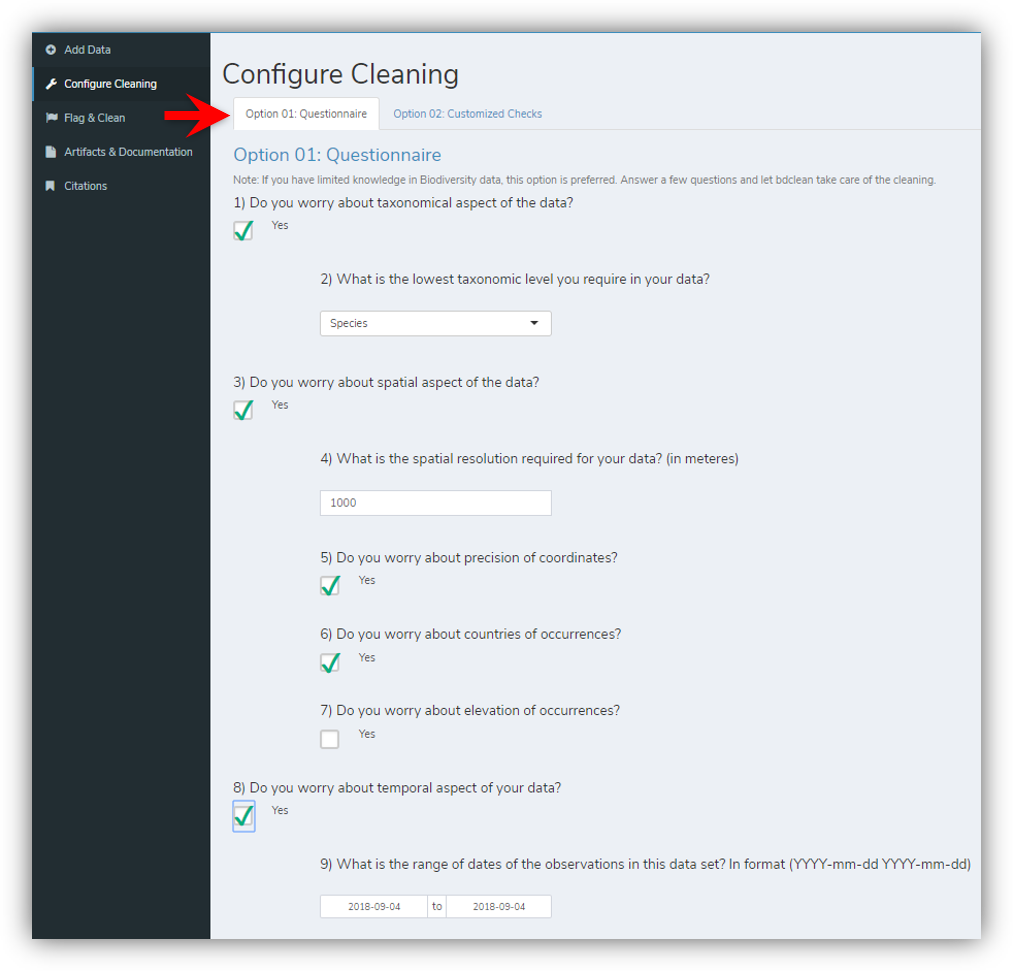
\includegraphics{img/bdclean_questionnaire-full.png}

\section{Option 2: choose data
checks}\label{option-2-choose-data-checks}

\begin{figure}
\centering
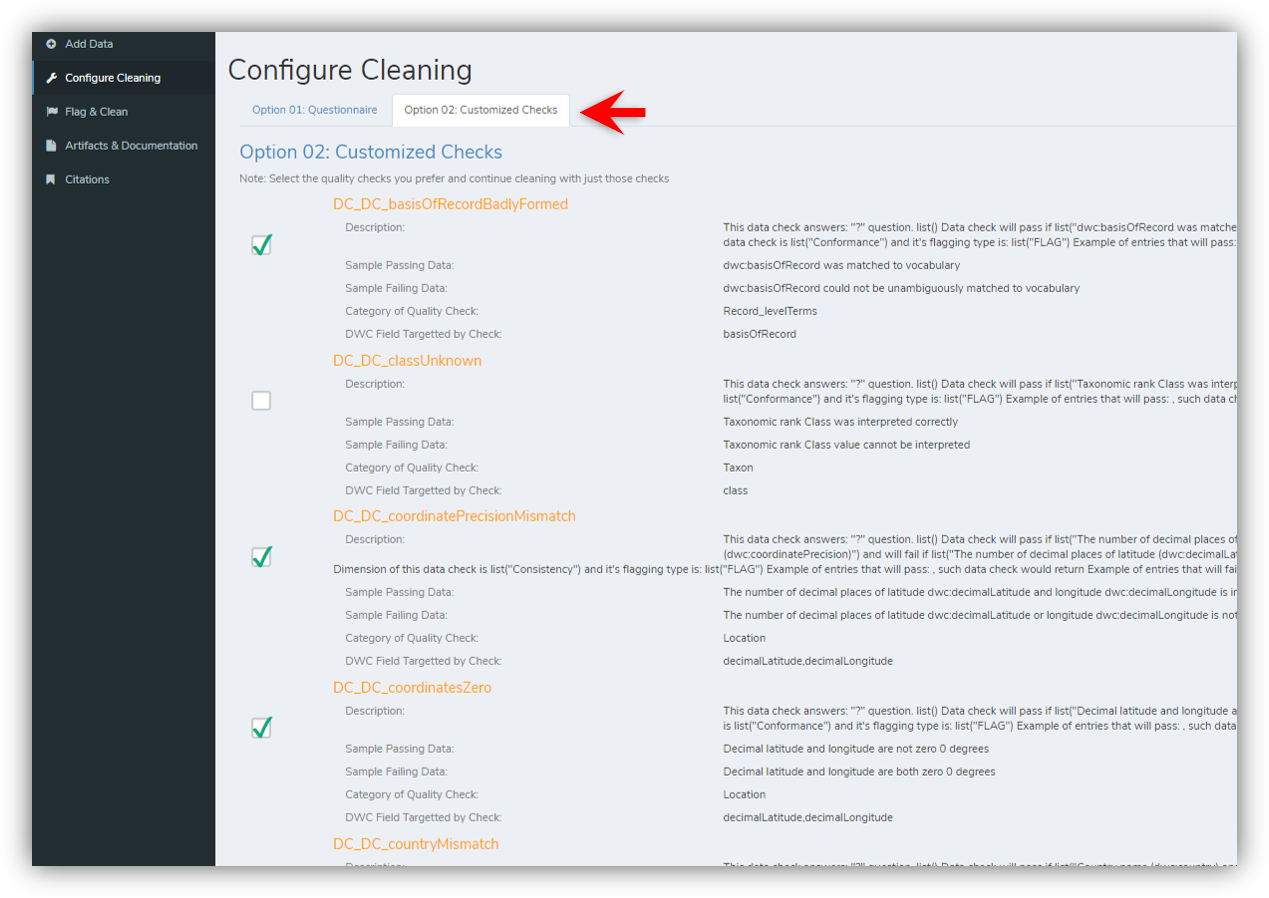
\includegraphics{img/bdclean_data-checks.png}
\caption{Choose your data checks}
\end{figure}

\chapter{Flaging and cleaning}\label{flaging-and-cleaning}

\begin{center}\rule{0.5\linewidth}{\linethickness}\end{center}

\section{Data flags}\label{data-flags}

\begin{figure}
\centering
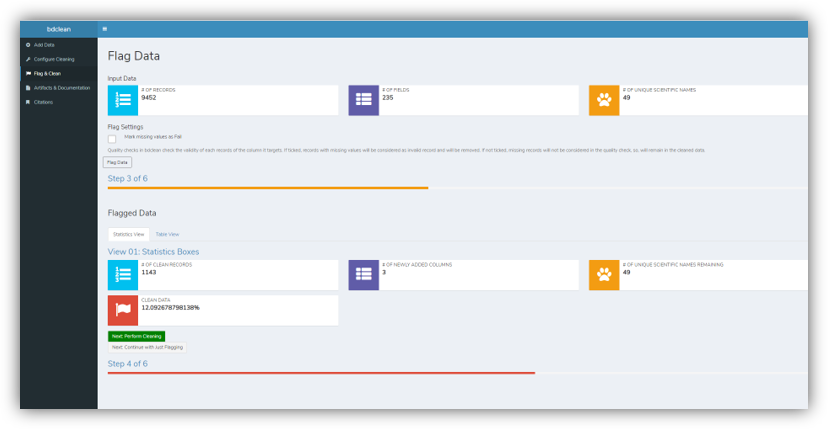
\includegraphics{img/bdclean_flag.png}
\caption{View flags}
\end{figure}

\section{Perform the cleaning}\label{perform-the-cleaning}

\begin{figure}
\centering
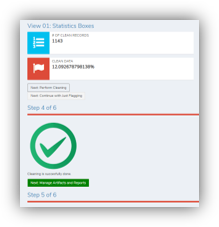
\includegraphics{img/bdclean_clean.png}
\caption{Perform the cleaning}
\end{figure}

\chapter{Artifacts and reports}\label{artifacts-and-reports}

\begin{center}\rule{0.5\linewidth}{\linethickness}\end{center}

\textbf{{{[} TBA {]}}}

\chapter{Getting your feedback}\label{getting-your-feedback}

\begin{center}\rule{0.5\linewidth}{\linethickness}\end{center}

Loading\ldots{}

\section{Report a bug}\label{report-a-bug}

Submit an issue at \url{https://github.com/bd-R/bdclean/issues}

\section{Contribute}\label{contribute}

Contribute: \url{https://github.com/bd-R/bdclean}

Join: \url{https://bd-r-group.slack.com}

\chapter{\texorpdfstring{\texttt{bdclean}
citation}{bdclean citation}}\label{bdclean-citation}

\begin{center}\rule{0.5\linewidth}{\linethickness}\end{center}

\begin{Shaded}
\begin{Highlighting}[]
\KeywordTok{citation}\NormalTok{(}\StringTok{"bdclean"}\NormalTok{)}
\end{Highlighting}
\end{Shaded}

\begin{verbatim}
## 
## To cite package 'bdclean' in publications use:
## 
##   Tomer Gueta, Thiloshon Nagarajah, Vijay Barve, Ashwin Agrawal,
##   Povilas Gibas and Yohay Carmel (2018). bdclean: A user-friendly
##   data cleaning app for the inexperienced R user. R package
##   version 0.1.900. https://github.com/bd-R/bdclean
## 
## A BibTeX entry for LaTeX users is
## 
##   @Manual{,
##     title = {bdclean: A user-friendly data cleaning app for the inexperienced R user},
##     author = {Tomer Gueta and Thiloshon Nagarajah and Vijay Barve and Ashwin Agrawal and Povilas Gibas and Yohay Carmel},
##     year = {2018},
##     note = {R package version 0.1.900},
##     url = {https://github.com/bd-R/bdclean},
##   }
\end{verbatim}

\chapter{Learn more about data
cleaning}\label{learn-more-about-data-cleaning}

\begin{center}\rule{0.5\linewidth}{\linethickness}\end{center}

\begin{itemize}
\item
  \textbf{\href{http://biodiversity-informatics-training.org/\%20target=\%22_blank\%22}{Biodiversity
  Informatics Training Curriculum (BITC)}}
\item
  \textbf{\href{http://biodiversity-informatics-training.org/webinar-series/\%20target=\%22_blank\%22}{BITC:
  Webinar Series}}
\item
  \textbf{\href{https://github.com/tdwg/dwc-qa/wiki/Webinars\%20target=\%22_blank\%22}{Darwin
  Core Hour webinar series}}
\item
  \textbf{\href{https://github.com/tdwg/dwc-qa/wiki\%20target=\%22_blank\%22}{The
  Darwin Core Questions \& Answers wiki}}
\item
  \textbf{\href{https://www.gbif.org/document/80509/principles-of-data-quality\%20target=\%22_blank\%22}{Principles
  of Data Quality} \citep{Chapman2005} }
\item
  \textbf{\href{https://journals.plos.org/plosone/article?id=10.1371/journal.pone.0178731\%20target=\%22_blank\%22}{A
  conceptual framework for quality assessment and management of
  biodiversity data} \citep{Veiga2017} }
\item
  \textbf{\href{http://dx.doi.org/10.1016/j.ecoinf.2016.06.001\%20target=\%22_blank\%22}{Quantifying
  the value of user-level data cleaning for big data: A case study using
  mammal distribution models} \citep{Gueta2016} }
\end{itemize}

\subsubsection*{References}\label{references}
\addcontentsline{toc}{subsubsection}{References}

\bibliography{bib/Veiga-2017.bib,bib/Chapman-2005.bib,bib/Gueta-2016.bib}


\end{document}
